\chapter{绪论}\label{chap1}

近十年来，基于神经网络（neural network）的深度学习（deep learning）技术凭借其卓越的任务性能与广泛的应用场景，已逐渐成为人工智能领域的支柱性技术，在计算机视觉\cite{he2016deep,ch-cv1}、自然语言处理\cite{DBLP:conf/nips/VaswaniSPUJGKP17,ch-nlp1}、智能推荐\cite{ch-re1}等领域实现了突破性进展。
然而，神经网络的 “黑盒” 特性始终制约着该技术的可信应用。
深度学习模型内部特征（feature）的提取与作用机制缺乏合理的理论解释，导致此类模型在安全攸关场景中的部署面临挑战，同时也使得深度学习的发展长期依赖经验驱动，缺乏先验的理论指导。

传统学习理论（learning theory）的分析范式深受统计学与最优化理论的影响，然而此类理论难以应对深度学习模型所具有的高维性、非线性和动态演化等特性所带来的挑战，其分析能力与深度学习应用的实际需求之间存在较大差异。
为弥补这一差异，一系列现代机器学习理论应运而生。
本文所关注的\textit{特征学习理论}
（Feature Learning Theory，FLT）\cite{DBLP:conf/nips/0006CBG22,DBLP:conf/focs/Allen-ZhuL21,DBLP:conf/iclr/Allen-ZhuL23,doi:10.1073/pnas.2421593122}便是其中的倍受关注的研究方向之一。
% \footnote{在本文中，FLT特指一类新兴的深度学习理论分支，而非广义上所有与特征相关研究的统称。为避免概念歧义，我们将在第 \ref{sec-related-works-learning-paradigms} 小节中明确FLT的内涵与外延，并探讨FLT与相关理论体系的异同。}
FLT致力于揭示神经网络从数据中提取、优化并利用特征的内在规律，为深度学习的可信性与可解释性提供理论支撑。
本章将首先阐述FLT的研究背景与意义，然后系统梳理国内外研究现状并明确本研究的主要目标与贡献，最后介绍论文的整体结构安排。

\section{研究背景与意义}

FLT作为深度学习领域的新兴基础理论，聚焦于揭示神经网络如何在学习算法的驱动下从数据中自动提取、优化并利用有效特征，其研究不仅具有深刻的学术理论价值，更对人工智能的高效、安全落地具有关键的指导意义。

\paragraph{FLT的理论价值}
首先，FLT对神经网络的诸多特有属性具有良好的解释能力。
相较于支持向量机、逻辑回归等传统机器学习模型，以卷积神经网络（Convolutional Neural Network, CNN）、自编码器（Autoencoder, AE）、Transformer（TF）等为代表的神经网络模型具备从图像、语音、视频等高维、多模态数据中自动提取有效特征的核心能力，从而在图像分类、自然语言处理等复杂任务中实现了性能的跨越式提升。
然而，人们对神经网络如何自动从数据中筛选、提取并利用特征等诸多核心问题缺乏系统性认知，这导致深度学习模型常被视为不可解释的黑盒子，严重阻碍了其理论发展与可信应用。
FLT通过数学建模、理论推导与实证分析，清晰刻画了模型结构、参数初始化与优化算法对特征学习过程的影响，揭示了诸多神经网络模型特有属性的内在机理（如良性过拟合\cite{DBLP:conf/nips/0006CBG22}（benign overfitting）、模型蒸馏\cite{DBLP:conf/iclr/Allen-ZhuL23}（model distillation）等），填补了传统理论与深度实践之间的鸿沟，为深度学习的可解释性提供了有力支撑。

此外，特征学习理论还为不同领域的机器学习问题提供了统一的理论分析框架。
在传统学习理论中，不同领域、场景下问题的分析框架一般也各自独立，所得结论无法相互参考比对。
特征学习理论的研究，能够提炼不同领域场景、不同数据与模型假设下特征提取、优化、迭代的共性规律，构建统一的理论分析框架，打破各研究方向的壁垒。
例如，特征学习理论可以在统一理论框架下分析并揭示知识蒸馏\cite{DBLP:conf/iclr/Allen-ZhuL23}、自监督对比学习\cite{DBLP:conf/icml/WenL21}与图神经网络学习\cite{DBLP:journals/corr/abs-2306-13926}等多个不同场景下的前沿问题的底层原理，实现理论认知在计算机视觉、自然语言处理、智能推荐等不同领域的跨场景迁移，推动机器学习理论体系的进一步系统化与完善化。

\paragraph{FLT对深度学习实践的指导意义}
在实践中，FLT可以指导深度学习模型的设计与优化。
传统深度学习模型设计多依赖研究者的经验与大量试错，具有封闭性与随机性的特点。
特征学习理论的研究成果，能够为模型结构设计、训练策略选择提供明确的理论指导。
例如，FLT研究揭示了“随机梯度下降法（Stochastic Gradient Descent, SGD）先挖掘后优化特征”的规律\cite{DBLP:conf/iclr/LuWYZ24}，由此可以针对性地优化模型训练的学习率调度策略；
基于“特征纯化提升鲁棒性\cite{DBLP:conf/focs/Allen-ZhuL21}” 的机理，研究者可改进对抗训练算法以增强模型的鲁棒性；“混合增强（Mixup）对特征学习的增益机制\cite{DBLP:conf/icml/ZouCLG23}”则给出了更高效的数据增强方案。上述三个例子均展示了FLT研究成果在深度学习模型设计与优化中的实际应用。

此外，FLT的研究还有助于提升模型的鲁棒性与泛化能力。
在深度模型的实际应用场景中，数据往往存在分布偏移、噪声干扰、样本稀缺等问题，对深度学习模型的泛化能力与鲁棒性提出了较高的需求。
FLT针对分布外泛化\cite{DBLP:journals/corr/abs-2304-11327,ch-ood1}（out-of-distribution generalization）、异常检验（anomaly detection）\cite{ch-rbad1,ch-rbad2}、小样本学习\cite{DBLP:conf/iclr/ChenDLG24}（few-shot learning）等场景的研究，能够帮助模型开发者从根本上理解的特征学习过程，进而提升模型的鲁棒性与泛化能力。
在上述示例中，FLT通过挖掘特征与真实任务标签的内在关联，抑制虚假特征的干扰；通过学习可迁移的通用特征，提升模型在未知数据分布下的泛化性能；通过特征多样化学习，缓解了小样本场景下的过拟合问题。
上述分析推动了AI模型在医疗影像诊断、工业质检、智能驾驶、金融风控等安全攸关领域的规模化落地，解决实际场景中的核心技术痛点。

\section{国内外研究现状}\label{sec-related-works}

特征，有时也被称作表示、表征（representation），广义上泛指数据在特定任务空间内的低维刻画，是一个跨越传统机器学习、深度学习与大语言模型（Large Language Model，LLM）时代的关键概念。
针对特征的研究始终是机器学习领域的核心热点之一，其研究范式与主要关注的问题也随着技术进步与时代变迁经历了深刻演变。
本节将从以下两个视角系统梳理国内外关于特征学习理论的研究现状：从横向对比FLT与相关研究范式、突出差异性；从纵向追踪FLT近年来的发展历程、总结其核心研究问题与主要研究成果。
由于该领域的研究发展较快，相关工作极其丰富，本文仅选择部分代表性成果进行讨论。

\subsection{学习理论的范式演变}\label{sec-related-works-learning-paradigms}

% 神经网络具备可以自动从数据中提取有效特征的能力，却也因此被视为 “黑盒” ；
% 关于神经网络特征学习机制的理论解释始终是学界研究的热点。
早期特征学习理论多基于统计学习理论（statistical learning theory）框架。
该框架数理基础坚实、分析过程严谨，衍生出诸多形式优美的理论成果。
Bengio等\cite{BCV2013Representation}的综述文章系统总结了包括概率PCA（Probabilistic Principal Component Analysis，PPCA）、受限玻尔兹曼机（Restricted Boltzmann Machine，RBM）、自编码器（Auto Encoders，AE）等模型的特征学习原理。
然而，早期特征学习理论始终受限于统计学习理论范式，研究重心集中于经验风险最小化（Empirical Risk Minimization, ERM）与归纳偏置（Inductive Bias）约束两大宏观优化目标，而对数据与模型间的匹配关系、神经元的微观动力学行为缺乏足够关注；以网络\emph{表示能力分析}（Expressiveness Analysis, EA）、\emph{VC维}（Vapnik-Chervonenkis Dimension, VCD）和\emph{样本复杂度}（Sample Complexity, SC）等为代表的早期理论框架无法分析神经网络的精细结构与特性，难以解释实践中所呈现的一系列神经网络特有现象。

随着深度学习技术的蓬勃发展，许多新型学习理论框架相继涌现，一些传统的理论框架也取得了若干新成果。
例如，\emph{神经正切核}（Neural Tangent Kernel, NTK）\cite{chntk-1}通过网络输出对参数梯度的内积定义核函数，在无限宽极限下将神经网络训练动态线性化为核回归问题，为超宽网络的收敛性与泛化性分析提供解析工具；
\emph{平均场理论}（mean field theory）以群体平均行为近似大规模系统中个体的复杂交互，将高维动力学降维为可解的自洽方程，适用于刻画神经网络特征学习动态或多智能体交互机制；
\emph{梯度流}（gradient flow）作为梯度下降的连续时间极限，通过常微分方程描述参数演化轨迹，是分析非凸损失曲面几何性质与优化收敛行为的核心框架；
另一方面，而作为传统学习理论的代表，\emph{概率近似正确}（Probably Approximately Correct，PAC）理论也被应用到了神经网络上。
该理论通过样本复杂度与置信度量化模型泛化能力，为算法的近似正确性提供概率保证，在深度学习时代也取得了若干新的研究成果。
我们在\cref{fig-learning-theory-taxonomy}中列举了当前机器学习领域若干主流的学习理论框架与各框架的相关研究成果。

2021年前后，Allen-Zhu与Li\cite{DBLP:conf/focs/Allen-ZhuL21,DBLP:conf/iclr/Allen-ZhuL23}提出了现代特征学习理论研究范式，并引发了学界的广泛关注与讨论。
如无特殊说明，本文中的“特征学习理论”一词或其英文缩写“FLT”特指这类新型研究范式；“早期特征学习”或“传统特征学习”一词则用来指代早期基于统计学习理论的研究。
鉴于FLT尚处于快速发展阶段，学术界对于FLT与其他理论方法的差异性及其核心研究问题的界定尚未达成一致共识。
为严谨起见，我们为本文所讨论的 FLT 作出如下界定。
\begin{mynote}{{\bfseries FLT}与其他理论框架的主要差异及其核心研究问题}
  \textit{本文所讨论的FLT是一类有限、离散，且算法相关的理论分析框架，主要用于分析具体学习任务（由数据集、模型类、模型评价标准与优化算法共同决定，参见\cref{sec-learning-task}）中模型参数的迭代规律。
  }
\end{mynote}
\noindent 其中，我们对有限、离散与算法相关这三大特性的解释如下：
\begin{itemize}
  \item \textbf{网络参数的有限性}：FLT以有限宽度网络为研究对象，并不要求网络宽度趋向无穷。相比NTK等无限维理论分析框架，FLT可以得到关于网络参数量（如网络宽度、卷积网络通道数等）的非渐近（non-asymptomatic）的结论，帮助研究者更深入地理解网络参数如何定量地影响网络的表现。
  \item \textbf{迭代过程的离散性}：FLT聚焦于模型参数的离散迭代优化过程，而非将其近似为连续的优化流。因此，FLT不同与梯度流、均值场理论等连续化分析框架，可以得到关于迭代步数的非渐近结论，且不需要对优化目标做过于理想化的假设。
  \item \textbf{结论的算法相关性}：FLT考虑具体学习算法对特征学习过程的影响，其所得结论与优化算法的特性相关。这与 PAC 学习、VC 维理论、表示性理论等传统学习理论的核心假设存在本质区别。
\end{itemize}
\cref{fig-learning-theory-taxonomy}展示了FLT与同时期其他常见学习理论分析框架的关系并突出了各理论框架在有限性、离散性与算法相关性上的差异。

\begin{figure}[htbp]
\centering
\iffastcompile
  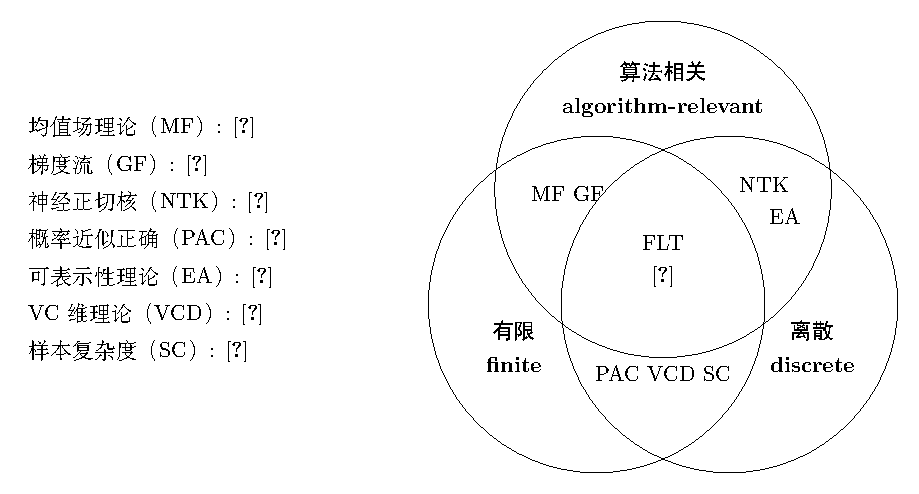
\includegraphics[width=0.99\textwidth]{figures/tikz/learning_theory_taxonomy.pdf}
\else
  \begin{tikzpicture}[scale=1.5]
  % 定义三个圆的中心
  \coordinate (A) at (0,0);
  \coordinate (B) at (1.5,0);
  \coordinate (C) at (0.75,1.3);

  % 画三个圆
  \draw[circle] (A) circle (1.9);
  \draw[circle] (B) circle (1.9);
  \draw[circle] (C) circle (1.9);

  % 标注圆的名称
  \node (finite) at ($(A)+(-0.6,-0.5)$) [above left] {\heiti{有限}};
  \node (finite_ref) at (finite.south) [below] {\textbf{finite}};
  \node (discrete) at ($(B)+(0.6,-0.5)$) [above right] {\heiti{离散}};
  \node (discrete_ref) at (discrete.south) [below] {\textbf{discrete}};
  \node (algorithm_relatedness) at ([yshift=12pt]$(C)+(0,0.7)$) [above] {\heiti{算法相关}};
  \node at (algorithm_relatedness.south) [below] {\textbf{algorithm-relevant}};

  % 圆之间的交集文字
  \node (PAC) at ($(A)!0.5!(B)+(0,-0.6)$) [below] {PAC\ VCD\ SC};
  \node (NTK) at ($(B)!0.5!(C)+(0.4,0.7)$) [right] {NTK};
  \node (EA) at ([xshift=-1pt,yshift=-10pt]NTK) [right] {EA};
  \node at ($(C)!0.5!(A)+(-0.35,0.6)$) [left] {MF\ GF};

  % 三圆交集文字
  \node (FLT) at ($(C)+(0,-0.6)$) {FLT};
  \node (FLT_ref) at (FLT.south) [below] {\cite{DBLP:conf/focs/Allen-ZhuL21}};

  % Caption
  \coordinate (caption1) at ($(A)+(-6.5,2)$);
  \node at (caption1) [right] {均值场理论（MF）: \cite{DBLP:conf/focs/Allen-ZhuL21}};
  \coordinate (caption2) at ([yshift=-12pt]caption1);
  \node at (caption2) [right] {梯度流（GF）: \cite{DBLP:conf/focs/Allen-ZhuL21}};
  \coordinate (caption3) at ([yshift=-12pt]caption2);
  \node at (caption3) [right] {神经正切核（NTK）: \cite{DBLP:conf/focs/Allen-ZhuL21}};
  \coordinate (caption4) at ([yshift=-12pt]caption3);
  \node at (caption4) [right] {概率近似正确（PAC）: \cite{DBLP:conf/focs/Allen-ZhuL21}};
  \coordinate (caption5) at ([yshift=-12pt]caption4);
  \node at (caption5) [right] {可表示性分析（EA）: \cite{DBLP:conf/focs/Allen-ZhuL21}};
  \coordinate (caption6) at ([yshift=-12pt]caption5);
  \node at (caption6) [right] {VC 维理论（VCD）: \cite{DBLP:conf/focs/Allen-ZhuL21}};
  \coordinate (caption7) at ([yshift=-12pt]caption6);
  \node at (caption7) [right] {样本复杂度（SC）: \cite{DBLP:conf/focs/Allen-ZhuL21}};
  \end{tikzpicture}
  \fi

  \caption{机器学习领域主流的理论框架示意图。左：各理论框架常见译名、英文缩写与相关参考文献。右：我们从算法相关性、有限性与离散性三个维度评价各理论框架对于不同学习任务的适用性，以突出FLT与其他理论框架的差异性。如第 \ref{sec-related-works-learning-paradigms} 小节所述，FLT 是一种算法相关、维度有限，且迭代过程离散的理论框架，适用于刻画神经网络的特征学习过程。}
  \label{fig-learning-theory-taxonomy}
\end{figure}

\subsection{FLT的研究进展}
\label{subsec: advance of FLT research}

FLT是一套面向实践应用的理论体系；凡是在实际训练、推理过程中神经网络表现出的性质、现象，都可作为FLT的分析对象与研究载体。
在 FLT 发展初期，研究者主要关注神经网络的一些普遍性质，例如良性过拟合的发生机制\cite{DBLP:conf/nips/0006CBG22}、SGD 算法的优化动力学机理 \cite{DBLP:conf/iclr/LuWYZ24}，以及对比学习（contrastive learning）范式下特征表征的学习机制与优化策略\cite{DBLP:conf/icml/WenL21}等。
在本文的\cref{chap3}，我们分析了对抗训练（adversarial training）的特征学习过程，并聚焦于\emph{特征塌缩}（neural collapse）这一普遍存在于神经网络最后一层特征中的性质。我们将标准训练的结论自然地推广到了对抗训练场景，并量化地分析了特征随对抗训练强度的变化规律及其对模型鲁棒性的影响。

随着与 FLT 相关探索的不断深入，关于神经网络共性的研究已日趋完善。
在此背景下，研究者的关注焦点开始转向更为细分、具体的实践场景或技术环节，例如知识蒸馏的特征迁移机制优化\cite{DBLP:conf/iclr/Allen-ZhuL23}、混合数据增强策略下的特征分布演化规律\cite{DBLP:conf/icml/ZouCLG23}等。
这类研究均旨在从细粒度层面挖掘特征学习的内在机理，为特定技术方案的优化提供理论支撑。
本文\cref{chap4}聚焦重构式异常检测（Reconstruction-Based Anomaly Detection, RBAD）场景下的特征学习动力学过程展开系统分析，最终证实：仅在正常数据上完成训练的生成式网络，在对异常样本进行重构时会产生显著更大的误差，基于这一特性可实现对异常点的有效检测。

随着大语言模型（Large Language Model，LLM）时代到来，关于语言模型（比如TF）与扩散模型（diffusion）的相关问题收到广泛的关注。
% TODO 多CITE一些FLT参考文献
本文基于神经网络研究了QA问题中的知识提取。

综上所述，本文紧跟国内外FLT的研究进展，针对对抗训练、异常检测与机器遗忘这三个学习任务中模型的特征学习机制展开分析。

\section{主要研究问题与技术路线}

在第 \ref{subsec: advance of FLT research} 小节中，我们总结了近几年FLT的研究进展，并
本研究计划围绕特征学习理论的核心科学问题（见\cref{sec-research-questions}），总结现有理论与与相关参考文献，建立统一的分析框架。
随后，我们聚焦对抗训练（adversarial training）、重构式异常检测（reconstruction-based anomaly detection, RBAD）、与LLM问答（question answering, QA）为例，深入考察神经网络在不同任务下的特征提取与演化机制，并总结归纳特征学习的共性特点与不同模型的适配机制。

\subsection{研究问题}\label{sec-research-questions}

本文主要关注下述三个特征学习领域的核心问题。
\begin{mynote}{本文的核心研究问题}
  \begin{itemize}
    \item 特征提取机制：神经网络如何自动从训练数据中提取有效特征？
    \item 特征演化机制：网络提取的特征如何随训练过程演化？
    \item 网络适配机制：为何特定结构的网络只能在一部分学习任务中表现出色？
  \end{itemize}
\end{mynote}
本文将围绕上述三个问题展开研究，并在第六章对每个问题给出简短的回答。

\subsection{技术路线}

\begin{figure}[htbp]
\begin{center}
\iffastcompile
    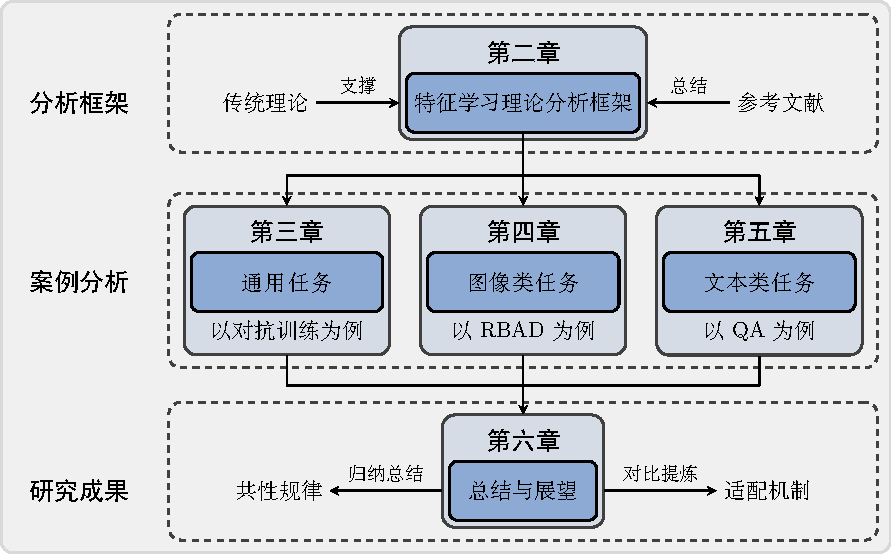
\includegraphics[width=0.99\textwidth]{figures/tikz/research_roadmap.pdf}
\else
    \begin{tikzpicture}[node distance=2cm]
        % 分析框架
        \node (top) [block] {特征学习理论分析框架};
        \node (top_caption) [above] at (top.north) {\zihao{-4}\heiti{第二章}};
        \begin{pgfonlayer}{bg3}
            \node (top_box) [draw=darkgray, fill=blue-background, line width=1pt, rounded corners=6pt, inner sep=0.1cm, fit=(top_caption) (top)] {};
        \end{pgfonlayer}
        \node (theory) [left] at ([xshift=-1.5cm]top.west) {传统理论};
        \node (ref) [right] at ([xshift=1.5cm]top.east) {参考文献};
        \draw [arrow] (theory.east) -- (top_box.west |- theory.east) node [above, midway] {\zihao{-5} 支撑};
        \draw [arrow] (ref.west) -- (top_box.east |- ref.west) node [above, midway] {\zihao{-5} 总结};
        \begin{pgfonlayer}{bg2}
            \node (topbox) [draw=darkgray, dashed, line width=1pt, rounded corners=6pt, inner sep=0.2cm, minimum width=12cm, align=center, fit=(theory) (top_box) (ref)] {};
        \end{pgfonlayer}

        % 案例分析
        \node (mid1) [block, below=of top, xshift=-4cm, text width=3cm] {通用任务};
        \node (mid1_caption) [above] at (mid1.north) {\zihao{-4}\heiti{第三章}};
        \node (mid1_task) [below] at (mid1.south) {以对抗训练为例};
        \begin{pgfonlayer}{bg3}
            \node (mid1_box) [draw=darkgray, fill=blue-background, line width=1pt, rounded corners=6pt, inner sep=0.1cm, fit=(mid1_caption) (mid1) (mid1_task)] {};
        \end{pgfonlayer}
        \node (mid2) [block, below=of top, text width=3cm] {图像类任务};
        \node (mid2_caption) [above] at (mid2.north) {\zihao{-4}\heiti{第四章}};
        \node (mid2_task) [below] at (mid2.south) {以RBAD为例};
        \begin{pgfonlayer}{bg3}
            \node (mid2_box) [draw=darkgray, fill=blue-background, line width=1pt, rounded corners=6pt, inner sep=0.1cm, fit=(mid2_caption) (mid2) (mid2_task)] {};
        \end{pgfonlayer}
        \node (mid3) [block, below=of top, xshift=4cm, text width=3cm] {文本类任务};
        \node (mid3_caption) [above] at (mid3.north) {\zihao{-4}\heiti{第五章}};
        \node (mid3_task) [below] at (mid3.south) {以QA为例};
        \begin{pgfonlayer}{bg3}
            \node (mid3_box) [draw=darkgray, fill=blue-background, line width=1pt, rounded corners=6pt, inner sep=0.1cm, fit=(mid3_caption) (mid3) (mid3_task)] {};
        \end{pgfonlayer}
    
        \begin{pgfonlayer}{bg2}
        \node (midbox) [draw=darkgray, dashed, line width=1pt, rounded corners=6pt, inner sep=0.2cm, minimum width=12cm, align=center, fit=(mid1_box) (mid2_box) (mid3_box)] {};
        \end{pgfonlayer}

        % 研究成果
        \node (bottom) [block, below=2.5cm of mid2] {总结与展望};
        \node (bottom_caption) [above] at (bottom.north) {\zihao{-4}\heiti{第六章}};
        \begin{pgfonlayer}{bg3}
            \node (bottom_box) [draw=darkgray, fill=blue-background, line width=1pt, rounded corners=6pt, inner sep=0.1cm, fit=(bottom_caption) (bottom)] {};
        \end{pgfonlayer}
        \node (modern_theory) [left] at ([xshift=-2cm]bottom.west) {共性规律};
        \node (application) [right] at ([xshift=2cm]bottom.east) {适配机制};
        \draw [arrow] (bottom_box.west |- modern_theory.east) -- (modern_theory.east) node [above, midway] {\zihao{-5} 归纳总结};
        \draw [arrow] (bottom_box.east |- application.west) -- (application.west) node [above, midway] {\zihao{-5} 对比提炼};
        \begin{pgfonlayer}{bg2}
            \node (bottombox) [draw=darkgray, dashed, line width=1pt, rounded corners=6pt, inner sep=0.2cm, minimum width=12cm, align=center, fit=(modern_theory) (bottom_box) (application)] {};
        \end{pgfonlayer}
    
        % 虚线框左上角加标题
        \coordinate (mid_caption) at ($(mid1.west) + (-3cm, 0)$);
        \coordinate (top_caption) at (mid_caption |- theory.west);
        \coordinate (bottom_caption) at (mid_caption |- bottom.west);
        \node (top_summary) [right, inner sep=2pt] at ([xshift=0.2cm]mid_caption) {\zihao{-4}\heiti{案例分析}};
        \node (mid_summary) [right, inner sep=2pt] at ([xshift=0.2cm]top_caption) {\zihao{-4}\heiti{分析框架}};
        \node (bottom_summary) [right, inner sep=2pt] at ([xshift=0.2cm]bottom_caption) {\zihao{-4}\heiti{研究成果}};
    
        % 第一层 -> 第二层
        \coordinate (mid_branch) at ($(mid2_box.north) + (0, 0.5cm)$);
        \coordinate (mid_branch_left) at ($(mid1_box.north) + (0, 0.5cm)$);
        \coordinate (mid_branch_right) at ($(mid3_box.north) + (0, 0.5cm)$);
        \draw [line] (top.south) -- (mid_branch);
        \draw [line] (mid_branch) -- (mid_branch_left);
        \draw [line] (mid_branch) -- (mid_branch_right);
        \draw [arrow] (mid_branch_left) -- (mid1_box.north);
        \draw [arrow] (mid_branch) -- (mid2_box.north);
        \draw [arrow] (mid_branch_right) -- (mid3_box.north);
    
        % 第二层 -> 第三层
        \coordinate (bottom_branch) at ($(mid2_box.south) + (0, -0.5cm)$);
        \coordinate (bottom_branch_left) at ($(mid1_box.south) + (0, -0.5cm)$);
        \coordinate (bottom_branch_right) at ($(mid3_box.south) + (0, -0.5cm)$);
        \draw [line] (mid1_box.south) -- (bottom_branch_left);
        \draw [line] (mid2_box.south) -- (bottom_branch);
        \draw [line] (mid3_box.south) -- (bottom_branch_right);
        \draw [line] (bottom_branch_left) -- (bottom_branch);
        \draw [line] (bottom_branch) -- (bottom_branch_right);
        \draw [arrow] (bottom_branch) -- (bottom_box.north);

        \begin{pgfonlayer}{bg1}
            \node (background) [draw=darkgray-background, fill=darkgray-background!40, line width=1pt, rounded corners=6pt, inner sep=0.2cm, minimum width=0.99\textwidth, align=center, fit=(topbox) (midbox) (bottombox) (mid_caption) (top_caption) (bottom_caption)] {};
        \end{pgfonlayer}
    \end{tikzpicture}
\fi
\end{center}
\end{figure}

\section{本文的主要贡献}

\section{论文结构安排}

本文共有六章，其中\cref{chap1}为绪论，介绍了特征学习理论的研究背景与意义，总结了该领域国内外发展近况，并概括了本文的研究内容与主要贡献。
在\cref{chap2}中，我们结合传统学习理论与现代深度学习的实际应用，总结出了适用于特征学习理论分析的统一分析框架。
在第\ref{chap3}至第\ref{chap5}章中，我们深入探讨了FLT在分析、阐释及优化深度学习实际应用问题中的具体作用与成效。
其中：
\begin{itemize}
  \item 第三章以对抗训练为研究场景，分析全连接神经网络特征学习动力学基础与神经塌缩特性，探究单纯形压缩现象的表征、成因及其与神经塌缩的关联差异，验证其对模型鲁棒性的影响。
  \item 第四章聚焦RBAD场景，探究图像数据与RBAD的适配性，构建卷积神经网络特征学习动力学模型，推导特征提取与数据重建的关联机制并开展实验验证。
  \item 第五章针对问答任务，构建Transformers知识提取动力学模型，解析自注意力机制驱动的知识捕捉与表达逻辑并验证其有效性。第六章对全文研究成果进行总结，分析研究局限性，并展望未来研究方向。
\end{itemize}
本文第\ref{chap3}到第\ref{chap5}章的分析始终围绕着我们在\cref{sec-research-questions}中提到的三个研究问题，即“网络如何自动提取有效特征”、“特征如何随训练过程演化”与“为何特定结构的网络在特定类型的数据上具有更优特征学习能力”。
在第六章，我们总结了全文的核心工作，为上述研究问题提供了一份详细的分析、回答。并就未来的潜在研究方向进行了深入思考。